\documentclass[zavrsnirad]{fer}
% Dodaj opciju upload za generiranje konačne verzije koja se učitava na FERWeb
% Add the option upload to generate the final version which is uploaded to FERWeb

\usepackage{blindtext}
\usepackage{listings}
\usepackage{hyperref}
\usepackage[dvipsnames]{xcolor}
\definecolor{darkgreen}{rgb}{0, 0.6, 0}

\lstdefinelanguage{CSharp}{
	language=[Sharp]C,
	morekeywords={
		abstract, as, base, bool, break, byte, case, catch, char, checked, class, const, continue,
		decimal, default, delegate, do, double, else, enum, event, explicit, extern, false, finally,
		fixed, float, for, foreach, goto, if, implicit, in, int, interface, internal, is, lock, long,
		namespace, new, null, object, operator, out, override, params, private, protected, public,
		readonly, ref, return, sbyte, sealed, short, sizeof, stackalloc, static, string, struct, switch,
		this, throw, true, try, typeof, uint, ulong, unchecked, unsafe, ushort, using, virtual, void,
		volatile, while, async, await, var, dynamic
	},
	sensitive=true,
	morecomment=[l]{//},
	morecomment=[s]{/*}{*/},
	morestring=[b]",
}

\lstdefinelanguage{GraphQL}{
	keywords={
		query, mutation, subscription, type, input, interface, union, scalar, enum, fragment, on,
		implements, extend, schema, directive, extends, null, true, false
	},
	keywordstyle=\color{blue}\bfseries,
	ndkeywords={
		__schema, __type, __typename, __directive, __inputValue, __field, __enumValue, __typeKind
	},
	ndkeywordstyle=\color{violet}\bfseries,
	sensitive=true,
	morecomment=[s]{""" }{ """},
	morecomment=[s]{"""}{"""},
	morestring=[b]{"},
	morestring=[s]{"""}{"""}
}

\lstdefinelanguage{Javascript}{
	keywords={typeof, new, true, false, catch, function, return, null, catch, switch, var, if, in, while, do, else, case, break},
	keywordstyle=\color{blue}\bfseries,
	ndkeywords={class, export, boolean, throw, implements, import, this, static, async},
	ndkeywordstyle=\color{purple}\bfseries,
	identifierstyle=\color{black},
	sensitive=false,
	comment=[l]{//},
	morecomment=[s]{/*}{*/},
	commentstyle=\color{purple}\ttfamily,
	stringstyle=\color{red}\ttfamily,
	morestring=[b]',
	morestring=[b]"
}

\lstset{
	basicstyle=\ttfamily,
	keywordstyle=\color{blue}\bfseries,
	commentstyle=\color{darkgreen}\itshape,
	stringstyle=\color{red},
	showstringspaces=false,
	numberstyle=\tiny\color{gray},
	numbersep=5pt,
	tabsize=2,
	breaklines=true,
	showtabs=false,
	showspaces=false,
	showlines=true,
	frame=single,
	backgroundcolor=\color{lightgray}
}

%--- PODACI O RADU / THESIS INFORMATION ----------------------------------------

% Naslov na engleskom jeziku / Title in English
\title{GraphQL-based server monitoring system}

% Naslov na hrvatskom jeziku / Title in Croatian
\naslov{Sustav za praćenje stanja poslužitelja temeljen na jeziku GraphQL}

% Broj rada / Thesis number
\brojrada{1234}

% Autor / Author
\author{Dominik Dejanović}

% Mentor 
\mentor{Prof.\@ Ivana Bosnić}

% Datum rada na engleskom jeziku / Date in English
\date{June, 2024}

% Datum rada na hrvatskom jeziku / Date in Croatian
\datum{lipanj, 2024.}

%-------------------------------------------------------------------------------


\begin{document}


% Naslovnica se automatski generira / Titlepage is automatically generated
\maketitle


%--- ZADATAK / THESIS ASSIGNMENT -----------------------------------------------

% Zadatak se ubacuje iz vanjske datoteke / Thesis assignment is included from external file
% Upiši ime PDF datoteke preuzete s FERWeb-a / Enter the filename of the PDF downloaded from FERWeb
\zadatak{hr_0036541578_73-1.pdf}


%--- ZAHVALE / ACKNOWLEDGMENT --------------------------------------------------

\begin{zahvale}
  % Ovdje upišite zahvale / Write in the acknowledgment
  Hvala na kavi...
\end{zahvale}


% Odovud započinje numeriranje stranica / Page numbering starts from here
\mainmatter


% Sadržaj se automatski generira / Table of contents is automatically generated
\tableofcontents


%--- UVOD / INTRODUCTION -------------------------------------------------------
\chapter{Uvod}
\label{pog:uvod}
Današnja tehnologija se iznimno oslanja na poslužitelje kako bi ostvarili razne funkcionalnosti koje su potrebne većini ljudi u svakodnevnom životu, od pretraživanje raznih web stranica i videa na internetu do povezanosti ogromnih mreža računala u virtualno \textcolor{red}{super-računalo}, poslužitelju su neophodni u tom procesu. 
\\Nažalost nije dovoljno konfigurirati poslužitelj za obavljanje određene zadaće i nadati se da će raditi zauvijek. Zbog raznih problema kao prirodne katastrofe, pogrešake u kodu, virusi i hakeri, neispravan rad komponenti, prevelikog broja zahtjeva te drugih problema koji se često događaju, može doći do usporenja poslužitelja, neispravnog obavljanja funkcionalnosti, te čak i do potpunog prestanka rada poslužitelja. Upravo zbog tih razloga postoji puno aplikacija koje se koriste za praćenje rada poslužitlja i obaviještavanje administratora u slučaju neispravnog rada. Problem koji se javalja kod velike većine ovakvih aplikacija je pregled specifičnog vremenskog perioda u kojem se dogodila greška, potreba za plaćanjem za naprednije funkcionalnosti aplikacije te pohranjivanje podataka samo u zadnjih nekoliko dana ili tjedana.
\\Cilj ove aplikacije je omogućiti praćenje jednog ili više poslužitelja kroz neograničen period vremena, što omogućava administratorima da pregledaju podatke o radu poslužitelja za specifični period vremena tijekom kojeg je nastala greška na poslužitelju.


%-------------------------------------------------------------------------------
\chapter{Funkcionalnosti}
\label{pog:opis_problema}
Aplikacije su namijenjene administratorima poslužitelja koji mogu:
\begin{itemize}
	\item dodati poslužitelje koji se prate
	\item konfigurirati poslužitelj:
	\begin{itemize}
		\item podesiti podatke koji (na primjer prate se podaci procesora, a podaci o pohrani ne)
		\item podesiti putanju na kojoj se nalazi API
		\item podesiti interval (u minutama) u kojem se šalju podaci na server
	\end{itemize}
	\item pregledati podatke o pojedinom poslužitelju
	\begin{itemize}
		\item pregledati podatke unutar određenog vremenskog perioda
		\item \textcolor{red}{zoomirati} i osvježiti pojedine grafove
	\end{itemize}
	\item pregledati obavijesti o poslužiteljima
\end{itemize}

%-------------------------------------------------------------------------------
\chapter{Korištene tehnologije}
\label{pog:koristene_tehnologije}
U ovom projektu su korištene razne tehnologije: RDBMS, web framework, backend tehnologije te brojne druge. U nastavku slijedi opis korištenih tehnologija.

\section{Linux}
Ovaj projekt je namijenjen za prikupljanje i prikaz podataka o poslužiteljima koji koriste Linux operacijski sustav. Razlog tome je sve veća popularnost linux u poslužitelja.
Koriste se razni linux programi za prikupljanje podataka kao:
\begin{itemize}
	\item  lscpu - podaci o procesoru
	\item top - podaci o trenutno pokrenutim procesima na operacijskom sustavu
	\item systemctl - podaci o određenom servisu kao trenutni status, lokacija, poruke te drugo
	\item lsblk -  podaci o diskovima i particijama na računalu
	\item journalctl - poruke koje je određeni servis poslao
\end{itemize}
Za programiranje i testiranje programa su korištene Arch Linux i Linux Mint distribucije, ali program bi trebao raditi na svim linux distribucijama, dokle god se na njih mogu instalirati potrebni programi za prikupljanje podataka i pokretanje aplikacija.

\section{GraphQL}
GrapQL je jezik korišten za dohvaćanje i slanje podataka na API. Odabran je GraphQL umjesto REST tehnologije zbog nekoliko prednosti koje GraphQL ima:
 \begin{itemize}
 	\item ugrađena validacija polja - ovo omogućava GraphQL-u da provjeri polja koja korisnik unosi tako da se ne treba ručno programirati provjeravanje polja (na primjer GraphQL će automatski izbaciti grešku ukoliko se u brojčano polje unese znakovni niz). Također podcrtava pogreške prilikom korištenja nepoznatih parametara i polja. Primjer koda preuzet sa  \url{https://graphql.org/learn/validation/}:
 	\begin{lstlisting}[language=GraphQL]
 		# INVALID: hero is not a scalar, so fields are needed
 		{
 			hero
 		}
 	\end{lstlisting}
 	\begin{lstlisting}[language=GraphQL]
 		{
 			"errors": [
 			{
 				"message": "Field \"hero\" of type \"Character\" must have a selection of subfields. Did you mean \"hero { ... }\"?",
 				"locations": [
 				{
 					"line": 3,
 					"column": 3
 				}
 				]
 			}
 			]
 		}
 	\end{lstlisting}
 	\item upiti slični SQL-u - za razliku od REST-a koji se oslanja na putanje, GraphQL koristi Query kako bi korisnik mogao pomoću određenih parametara filtirati podatke te odabrati koje podatke želi dohvatiti
 	\item dohvaćanje više podataka u jednom zahtjevu - koristeći REST, korisnik bi morao za dohvaćanje raznih podataka slati puno upita, dok se u GraphQL-u može dohvatiti proizvoljan broj nepovezanih podataka u jednom zahtjevu. Primjer koda preuzet sa \url{https://graphql.org/learn/queries/}
 	\begin{lstlisting}
 		{
 			empireHero: hero(episode: EMPIRE) {
 				name
 			}
 			jediHero: hero(episode: JEDI) {
 				name
 			}
 		}
 	\end{lstlisting}
 	\begin{lstlisting}[language=GraphQL]
 		{
 			"data": {
 				"empireHero": {
 					"name": "Luke Skywalker"
 				},
 				"jediHero": {
 					"name": "R2-D2"
 				}
 			}
 		}
 	\end{lstlisting}
 \end{itemize}

\section{HotChocolate}
\label{pog:hotchocolate}
HotChocolate je implementacija GraphQL poslužitelja u C\# programskom jeziku. Ona nam omogućava korištenje svih funkcionalnosti GraphQL tehnologije bez da ih moramo ručno implementirati.\\Korištena verzija: 13.6.0
\begin{figure}[htb]
	\centering
	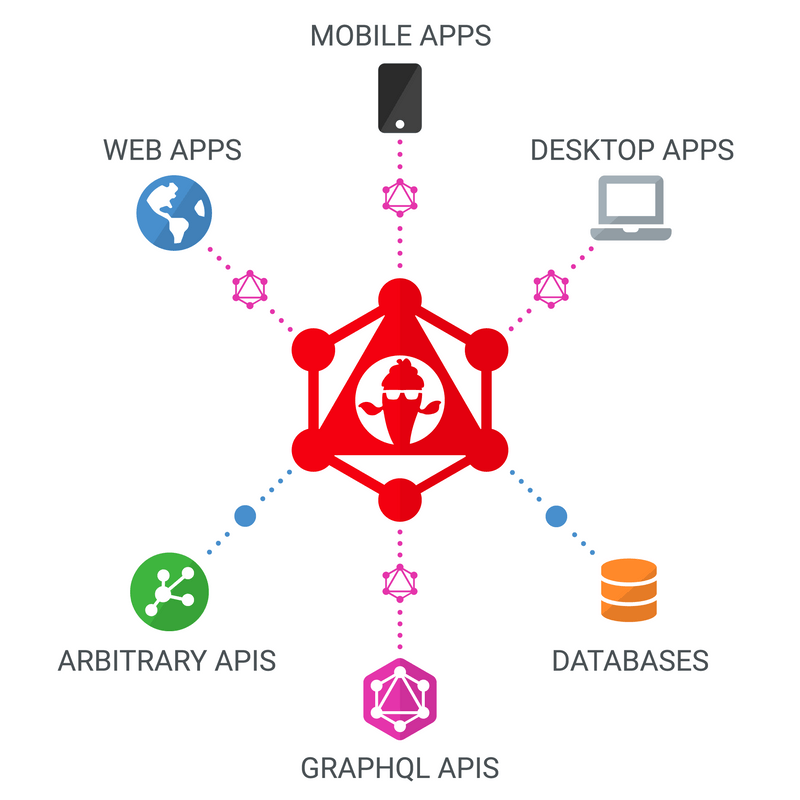
\includegraphics[width=0.6\linewidth]{images/hot_chocolate.png} 
	\caption{HotChocolate server}
	\label{slk:hot_chooclate}
\end{figure}
\\\textcolor{red}{ADD IMAGE REFERENCE} https://chillicream.com/static/cfd2ddde71f95ed876541f87c15b2a08/78d47/platform.png\\https://chillicream.com/docs/hotchocolate/v13

\section{.NET i C\#}
Za programiranje API-a i Monitor-a se koristi C\# programski jezik i .NET framework.\\
Korištena .NET verzija: net8.0\\Korištena C\# verzija: 12.0

\section{linq2db}
\label{pog:linq2db}
linq2db paket se koristi za pretvaranje LINQ koda u SQL kod kako bi se moglo lako pristupati bazi podataka.
\\Nakon instalacije paketa se pomoću određenih naredbi može spojiti na bazu podataka i iz nje generirati C\# klase koje odgovaraju tablicama u bazi podataka:
\begin{lstlisting}[language=CSharp]
	using System;
	using LinqToDB.Mapping;
	
	[Table("Products")]
	public class Product
	{
		[PrimaryKey, Identity]
		public int ProductID { get; set; }
		
		[Column("ProductName"), NotNull]
		public string Name { get; set; }
		
		[Column]
		public int VendorID { get; set; }
		
		[Association(ThisKey = nameof(VendorID), OtherKey=nameof(Vendor.ID))]
		public Vendor Vendor { get; set; }
		
		// ... other columns ...
	}
\end{lstlisting}
linq2db repozitorij: \url{https://github.com/linq2db/linq2db}

\section{Newtonsoft.Json}
Koristi se za serijalizaciju i deserijalizaciju JSON podataka.
Newtonsoft.Json repozitorij: https://github.com/JamesNK/Newtonsoft.Json

\section{Vue.js}
\label{pog:vue}
Vue.js je Javascript framework, koristi se za jednostavniji rad sa prikazom podataka i za bolje strukturiranje koda.
Primjer Vue koda za povećanja vrijednosti gumba nakon klika (preuzeto sa \url{https://vuejs.org/guide/introduction.html}):
\begin{lstlisting}[language=html]
	<div id="app">
	<button @click="count++">
	Count is: {{ count }}
	</button>
	</div>
\end{lstlisting}
Korištena verzija: 3.2.13
\\Vue.js dokumentacija: \url{https://vuejs.org/guide/introduction.html}

\subsection{primevue}
Primevue sadržava razne Vue komponente koje se koriste za dinamički prikaz podataka na ekranu (prilikom promijene podataka se odmah mijenja i prikaz bez potrebe za dodatnim kodom). Također se koristi primeicons biblioteka koja omogućuje korištenje raznih ikona.
\\Korištena primevue verzija: 3.52.0
\\Korištena primeicons verzija: 7.0.0
\\Dokumentacija: \url{https://primevue.org/}

\subsection{vue-chartjs}
\label{pog:chart.vue}
vue-chartjs je Vue biblioteka koja se koristi za prikaz grafova ovisno o predanim parametrima.
\\Korištena verzija: 5.2.0
\\Dokumentacija: \url{https://vue-chartjs.org}

\subsection{vue-datepicker}
vue-datepicker je Vue komponenta koja se koristi za odabir datuma i vremena.
\\Korištena verzija: 7.1.0
\\Dokumentacija: \url{https://vue3datepicker.com/}

\section{PostgreSQL}
\label{pog:postgresql}
Odabran je PostgreSQL kao RDBMS sustav za upravljanje bazom podataka zato što je otvorenog koda te ima opširnu dokumentaciju i korisničku podršku.
\\Korištena verzija: 16.2
\\PostgreSQL dokumentacija: \url{https://www.postgresql.org/docs}

\section{Git i Github}
Git je korišten kao sustav za praćenje verzija koda. Također je korišten Github koji omogućava pristup kodu i uputama za instalaziju.
\\Službena git stranica: \url{https://git-scm.com}
\\Github: \url{https://github.com/}


%-------------------------------------------------------------------------------
\chapter{Opis rješenja}
\label{pog:opis_rjesenja}
\section{\textcolor{red}{Softver}}
Napravljene su tri .NET projekta (API, Common i Monitor), web stranica te baza podataka.
\\API je centralna aplikacija koja povezuje Monitor i web stranicu s bazom podataka. To je ostvareno pomoću GraphQL-a, kod kojeg se koristi Query objekt za dohvaćanje podatka za web stranicu, te Mutation objekti koji se koriste kako bi Monitor mogao pisati podatke u bazu podataka.
\\Monitor je aplikacija koja se pokreće na poslužitelju koji se prati. Ona u specificiranom intervalu prikuplja razne podatke o poslužitelju te ih šalje API-u koji ih zapisuje u bazu podataka.
\\Web stranica se zatim koristi za prikaz prikupljenih podataka o pojedinačnim serverima, te za prikaz obavijesti i upozorenja koje je API generirao prilikom upisa podataka u bazu podataka.

\section{\textcolor{red}{Fizička konfiguracija}}
Postoji jedan centralni poslužitelj na kojem su pokrenute dvije aplikacije: Vue web stranica te API. Vue web stranica se dohvaća HTTP protokolom, nakon čega ona šalje zahtijeve API aplikaciji na centralnom poslužitelju radi dohvata podataka iz baze podataka.
\\Poslužitelji koji su konfigurirani za praćenje podataka također komuniciraju sa API aplikacijom, ali ne za dohvaćanje nego za slanje podataka API-u koji onda te podatke sprema u bazu podataka.
\begin{figure}[htb!]
	\centering
	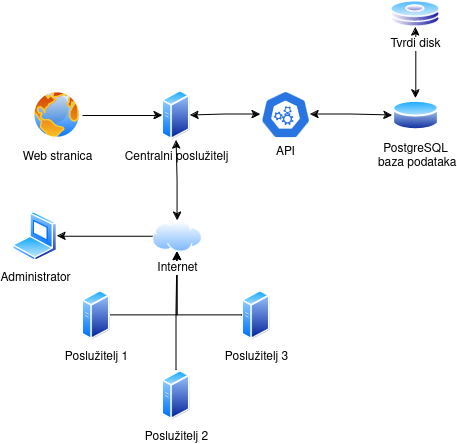
\includegraphics[width=0.6\linewidth]{images/flowchart.png} 
	\caption{Dijagram rješenja}
	\label{slk:flowchart}
\end{figure}
\\U nastavku slijedi detaljan opis funkcionalnosti i koda svih projekata.

\chapter{Baza podataka}
Za izradu baze podataka je korišten \ref{pog:postgresql} Postgresql. U korijenskoj strukturi repozitorija se nalazi datoteka db.sql pomoću koje se stvara baza podataka. U nastavku je opisana struktura baze podataka.
\begin{figure}[htb!]
	\centering
	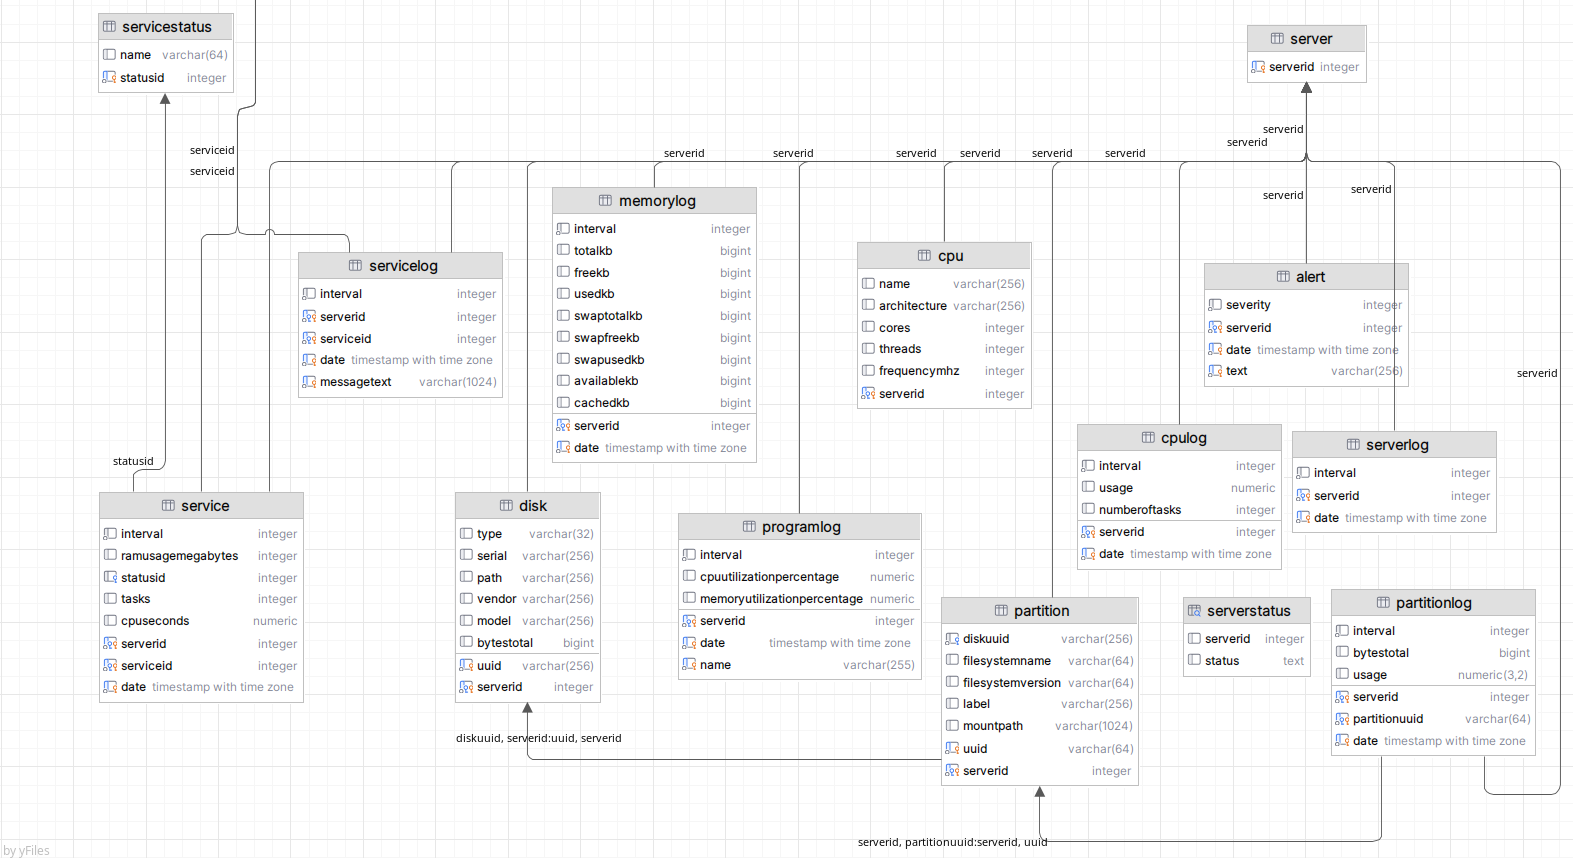
\includegraphics[width=1.15\linewidth]{images/db_structure.png} 
	\caption{Struktura baze podataka}
	\label{slk:db_structure}
\end{figure}

\section{Poslužitelj}
Za praćenje poslužitelja se koristi tablica server koja samo pohranjuje ID poslužitelja. Ovu tablicu referencira većina drugih tablica.
\\Također je napravljen jedan pogled koji se koristi za dohvat statusa poslužitelja. Poslužitelj se smatra aktivnim ako je od zadnjeg slanja podataka prošlo manje od n minuta (n = interval specificiran prilikom zadnjeg slanja podataka).
\lstinputlisting[firstline=16,lastline=22,language=SQL,title=serverStatus pogled]{db.sql}

\section{Procesor}
Za praćenje podataka o procesoru se koriste tablice cpu i cpulog. Tablica cpu pohranjuje općenite podatke o procesoru: ime procesora (name), arhitektura (architecture), broj jezgri (cores), broj niti (threads), frekvencija rada (frequency) te poslužitelj kojem on pripada (serverId).
\\cpulog tablica sprema podatke o procesoru koji se mijenjaju tijekom vremena kao iskorištenost procesora (usage) i broj procesa koje on obrađuje (numberoftasks).

\section{Priručna memorija}
Za pohranjivanje podataka o priručnoj memoriji se koristi samo tablica memorylog koja pohranjuje podatke o datumu prikupljanja podataka (date) ukupnoj memoriji (totalkb, freekb, usedkb), "swap" memoriji (swaptotalkb, swapfreekb, swapusedkb), neiskorištenoj memoriji (availablekb), "cache" memoriji (cachedkb), te ID poslužitelja kojem memorija pripada.
\\Za razliku od procesora, ne koristi se zasebna tablica za pohranu općenitih podataka o priručnoj memoriji kao proizvođač, serijski broj te drugo, jer nije pronađen način da se ti podaci očitaju sa poslužitelja bez administratorskih privilegija.

\section{Trajna pohrana}
Za pohranu trajne memorije se koriste tablice:
\begin{itemize}
	\item disk - općenite informacije o tvrdom disku: jedinstveni ID (uuid), tip (type), serijski broj (serial), putanja na kojoj se disk nalazi (path), proizvođač (vendor), model, veličina diska (bytestotal) i ID poslužitelja na kojem se disk nalazi
	\item partition - općenite informacije o jednoj particiji: jedinstveni ID (uuid), UUID diska kojem pripada (diskuuid), tip i verzija datotečnog sustava (filesystemname, filesystemversion), naziv particije (label), putanja na kojoj se nalazi (mountpath) te ID poslužitelja na kojem se particija nalazi
	\item partitionlog - podaci o particiji koji se mijenjaju tijekom vremena kao veličina particije (bytestotal) te iskorištenost (usage)
\end{itemize}

\section{Servisi}
Servisi nisu do kraja implementirani u aplikaciji, no podloga za praćenje podataka o servisima je implementirana su u bazi podataka. Za praćenje servisa se koriste tablice:
\begin{itemize}
	\item service - prikupljeni podaci o statusu servisa kao pohrana koju koristi (ramusagemegabytes), broj procesa koje je servis stvorio (tasks), procesorska snaga koju koristi (cpuseconds) te status servisa (statusid)
	\item servicename - \textcolor{red}{mapira} jedinstveni broj u naziv servisa
	\item servicelog - pohranjuje poruke koje je servis poslao (messagetext) te vrijeme kada su poslane (date)
	\item servicestatus - \textcolor{red}{mapira} id statusa servisa u tekstualnu reprezentaciju
\end{itemize}

\section{Programi}
Podška za programe nije do kraja implementirana u aplikaciji, no podloga za njihovo praćenje je implementirana su u bazi podataka.
\\Za praćenje programa se koristi tablica programlog koji pohranjuje  neke podatke kao ime programa (name) te postotak procesora (cpuutilizationpercentage) i memorije (memoryutilizationpercentage) koju program koristi.

\section{Obavijesti}
Stvorena je tablica za obavijesti koja pohranjuje \textcolor{red}{kritičnost} poruke (severity), ID poslužitelja za koji je relevantna (serverid) te datum (date) i tekst poruke (text).
\\Uz tablicu je također napravljena i metoda before\_alert\_insert\_func() koja se poziva prije unosa podataka u tablicu. Metoda je stvorena kako bi se onemogućio unos iste obavijesti ako je ona već poslana u zadnjih sat vremena (na primjer ako se proba unijeti "Server 0 cpu load above 90\%" u razmaku od 30 minuta, ta poruka će biti zapisana samo prvi put u bazu podataka, a drugi put se odbacuje uz grešku).
\lstinputlisting[firstline=172,lastline=176,language=SQL,title=before\_alert\_insert\_func()]{db.sql}

\chapter{API}
API aplikacija je implementirana koristeći \ref{pog:hotchocolate} HotChocolate server paket koji implementira funkcionalnosti GraphQL poslužitelja.
\\Struktura projekta:
\begin{figure}[htb]
	\centering
	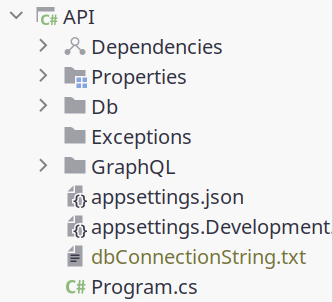
\includegraphics[width=0.4\linewidth]{images/api_structure.png} 
	\caption{Struktura API projekta}
	\label{slk:api_structure}
\end{figure}

\section{Program.cs}
Program.cs je datoteka koja se pokreće prilikom pokretanja programa. Glavne funkcije koje ona izvršava su konfiguracija Dependency Injectiona te mapiranje putanja API-a.
\\Dependency Injection je način strukturiranja koda kod kojeg se klase ne stvaraju direktno pomoću kodne riječi "new" nego se parametri konstruktora klase automatski predaju u nju. Odabran je ovaj način izrade koda kako bi se omogućilo lagano testiranje koda u budućnosti jer se umjesto stvarne klase koja obavlja određenu funkcionalnost može predati lažna klasa koja emulira stvarnu klasu (na primjer kao "IDb database" sučelje se umjesto klase koja obavlja funkcionalnolsti stvarne baze podataka predaje lažna klasa koja samo provjerava da li je određena metoda pozvana tri puta; ako da onda je test ispravan a u suprotnom je neispravan).

\section{GraphQL direktorij}
\label{pog:graphql_dir}
GraphQL direktorij sadržava sav kod potreban za ispravan rad GraphQL poslužitelja kao Query i Mutation kodovi te kod za rad sa obavijestima.

\begin{figure}[htb!]
	\centering
	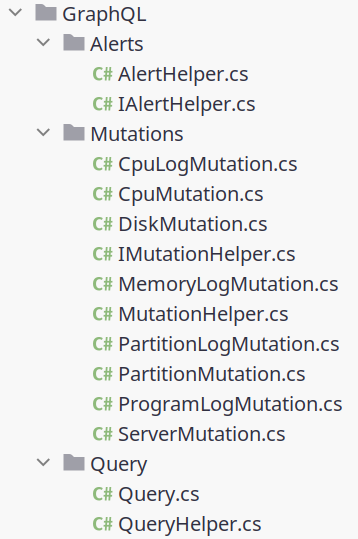
\includegraphics[width=0.5\linewidth]{images/graphql_dir_structure.png} 
	\caption{Struktura GraphQL direktorija}
\label{slk:graphql_dir_structure}
\end{figure}

\subsection{Query.cs}
\label{pog:query.cs}
Koristi se za dohvat podataka iz baze podataka. Za svaki tip podatka (CPU, memorija, tvrdi disk, ...) je napravljena metoda koja se poziva kada korisnik šalje zahtjev pomoću kojega se pokušava dohvatiti određen podatak.
\\Svaka metoda predstavlja tip query objekta koji se pokušava dohvatiti, a svi parametri te metode predtavljaju argumente koje korisnik specificira tijekom slanja zahtjeva.
\\Neki od parametara koje gotova svaka metoda ima su:
\begin{itemize}
	\item serverId - dohvaćaju se samo podaci koje je poslao server čiji je ID jednak ovom argumentu
	\item startDateTime - dohvaćaju se samo podaci poslani nakon specificiranog datuma i vremena
	\item endDateTime - dohvaćaju se samo podaci poslani prije specificiranog datuma i vremena
\end{itemize}
Klasa se oslanja na \ref{pog:db_dir} IDbProvider sučelje za rad sa bazom podataka, te na metodu \ref{GetLogs} GetLogs metodu za dohvat \textcolor{red}{logova} iz baze podataka.
\\Primjer jedne takve metode:
\lstinputlisting[language=CSharp, title=Cpu metoda, firstline=21, lastline=48]{API/GraphQL/Query/Query.cs}

\subsection{QueryHelper.cs}
Pomoćna klasa koju koristi \ref{pog:query.cs} Query.cs klasa. Sastoji se od raznih metoda od kojih je najbitnija GetLogs metoda koja sadržava algoritam koji se koristi za spajanje više podataka u jedan. Algoritam radi tako da pomoću početnog i zadnjeg datuma izračuna interval unutar kojeg se podaci spajaju u jedan:
\begin{lstlisting}[language=CSharp, title=Izračun intervala]
return (int)((DateTime)endDate).Subtract((DateTime)startDate).TotalHours;
\end{lstlisting}

Nakon izračuna intervala se dohvačaju podaci iz tablice koji su pohranjeni nakon specificiranog početnog datuma i prije krajnjeg datuma. Nakon toga se prolazi kroz svaki podatak te se koristi \ref{pog:dataset_helper} DatasetHelper klasa za spajanje više podataka u jedan, te se na kraju list spojenih podataka vraća.

\lstinputlisting[language=CSharp, title=Parametri GetLogs metode, firstline=99, lastline=105,label=GetLogs]{API/GraphQL/Query/QueryHelper.cs}

\subsection{DatasetHelper.cs}
\label{pog:dataset_helper}
Pomoćna klasa korištena u algoritmu spajanja više podataka u jedan podatak. Najvažnija metoda u klasi je AddLog metoda koja dodaje podatak u listu podataka koja se kasnije vraća. Broj podataka koji se spaja u jedan podatak ovisi o intervalu. Na primjer ako je interval 30, a podaci se bilježe svakih 5 minuta, spaja se 6 podataka u jedan. Ako je došlo do prekida u slanju podataka (na primjer podaci se šalju svakih 5 minuta, ali jedan podatak se pošalje nakon 7 minuta), onda se za period između ta dva podatka vraća "prazan" podatak koji signalizira prekid u slanju podataka. Algoritam radi na ovaj način kako bi se korisnike moglo obavijestiti ukoliko je došlo do prekida slanja podataka.
\lstinputlisting[language=CSharp, firstline=20, lastline=50, title=AddLog metoda]{API/GraphQL/Query/DatasetHelper.cs}

\subsection{Mutations direktorij}
Sadržava klase i sučelja koja se koriste za dodavanje i osvježavanje podataka u bazi podataka.
\\Važnije klase i sučelja u direktoriju:
\begin{itemize}
	\item IMutationHelper - sučelje koje definira funkcionalnosti koje su potrebne za umetanje, osvježavanje i brisanje pojedinačnih ili liste podataka iz baze podataka
	\item MutationHelper - implementacija IMutationHelper sučelja
\end{itemize}
Primjer dijela jedne mutacije:
\lstinputlisting[language=CSharp, firstline=10, lastline=24, title=CpuMutation.cs]{API/GraphQL/Mutations/CpuMutation.cs}

\subsection{IAlertHelper.cs}
Koristi se za slanje obavijesti bazi podataka.
\lstinputlisting[language=CSharp, firstline=5, title=IAlertHelper.cs]{API/GraphQL/Alerts/IAlertHelper.cs}

\section{Db direktorij}
\label{pog:db_dir}
Db direktorij sadržava sve pomoćne klase i modele koji se koriste za interakciju sa bazom podataka. Većina klasa u direktoriju Models su automatski generirane (i djelomično ručno promijenjene) korištenjem \ref{pog:linq2db} linq2db paketa pomoću naredbe "dotnet linq2db scaffold -p PostgreSQL -c "Host=localhost; Username=[username];\\Password=[password];Database=[database]""

\begin{figure}[htb!]
	\centering
	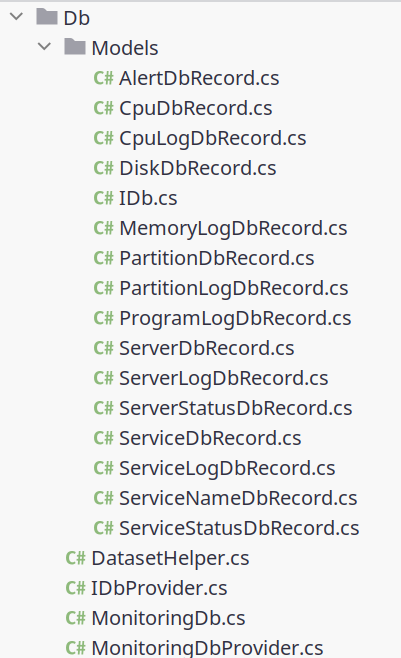
\includegraphics[width=0.5\linewidth]{images/db_dir_structure.png} 
	\caption{Struktura Db direktorija}
	\label{slk:db_dir_structure}
\end{figure}

Neke od važnijih klasa (te one koje nisu automatski generirane):
\begin{itemize}
	\item Models/IDb.cs - sučelje koje sadržava popis svih tablica u bazi podataka
	\lstinputlisting[language=CSharp,firstline=6]{API/Db/Models/IDb.cs}
	\item MonitoringDb.cs - automatski generirana implementacija IDb.cs sučelja
	\item MonitoringDbProvider.cs - koristi se za generiranje nove konekcije na bazu podataka (potrebno jer se koristi Dependency Injection)
\end{itemize}

\section{Konfiguracijske datoteke}
U programu se nalaze tri konfiguracijske datoteke: appsetting.json, appsettings.Development.json i dbConnectionString.txt od kojih će samo zadnja biti opisana.
\\dbConnectionString.txt datoteka sadržava niz znakova koji se koristi za spajanje na postojeću bazu podataka prilikom pokretanja programa:
\begin{lstlisting}[title=dbConnectionString.txt]
	Host=localhost;Username=[username];Password=[password];Database=[dbName];Include Error Detail=[true for debugging; false for deployment]
\end{lstlisting}

\section{Pokretanje API-a}
API se pokreće iz komandne linije/terminala pomoću naredbe "dotnet run" unutar direktorija u kojem se API nalazi.
\\Nakon pokretanja se može pristupiti URL-u \url{http://localhost:3000//graphql}, prilikom čega se otvara web stranica na kojoj se može vidjeti dokumentacija API-a te se mogu izvršavati upiti.
\begin{figure}[htb!]
	\centering
	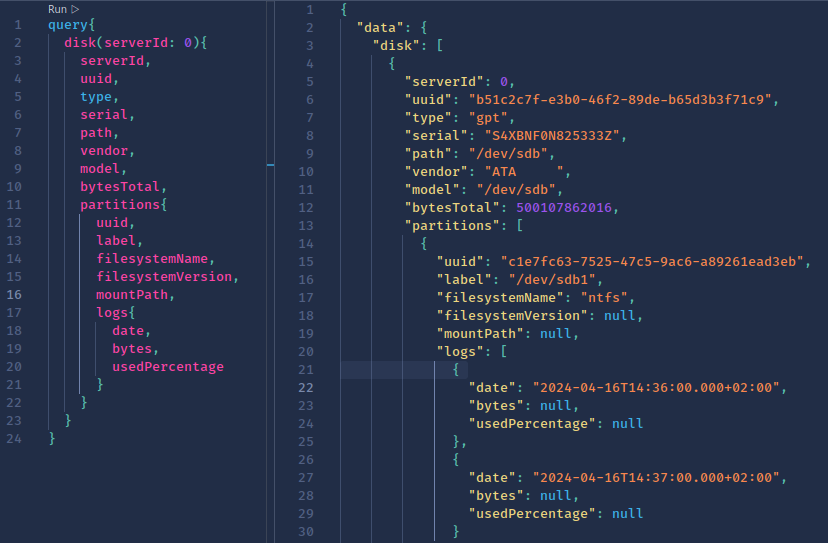
\includegraphics[width=1\linewidth]{images/api_query.png} 
	\caption{Dohvat podataka o pohrani}
	\label{slk:api_query}
	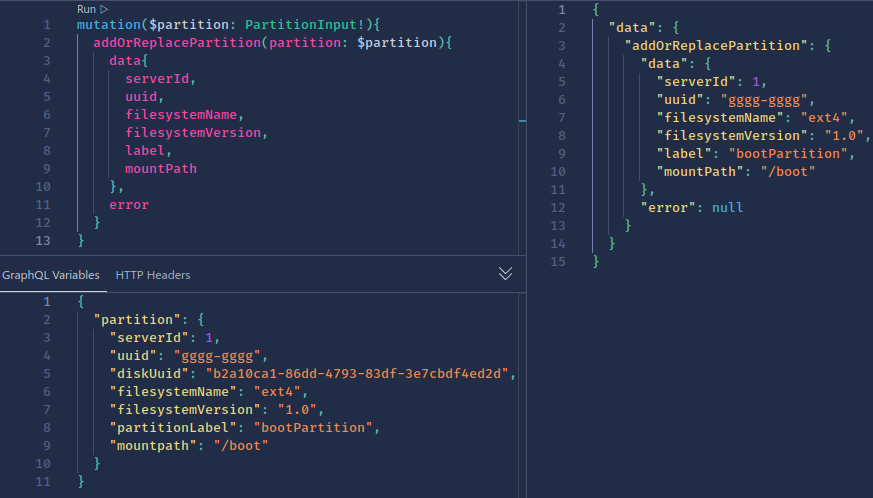
\includegraphics[width=1\linewidth]{images/api_mutation.png} 
	\caption{Dodavanje jedne particije}
	\label{slk:api_mutation}
\end{figure}

\chapter{Monitor}
Aplikacija Monitor se koristi za prikupljanje podataka o poslužitelju te slanje tih podataka API-u.

\begin{figure}[htb!]
	\centering
	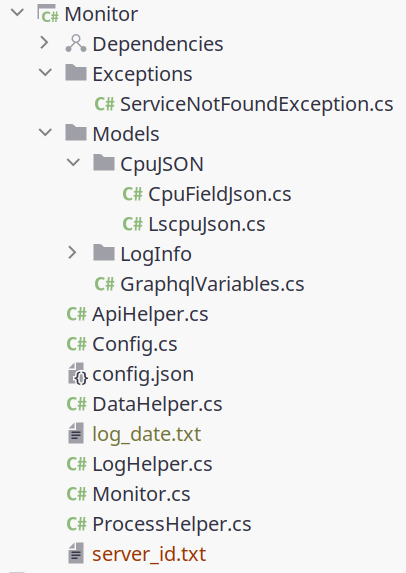
\includegraphics[width=0.4\linewidth]{images/monitor_structure.png} 
	\caption{Struktura Monitor projekta}
	\label{slk:monitor_structure.png}
\end{figure}

Objašnjenje važnijih dijelova aplikacije
\begin{itemize}
	\item Monitor.cs - pokreće se prilikom pokretanja aplikacije
	\item Models direktorij - sadržava klase koje se koriste za serijalizaciju i deserijalizaciju podataka dohvaćenih sa terminala
	\item ApiHelper.cs - koristi se za slanje podataka API-u
	\item config.json - koristi ju korisnik kako bi konfigurirao aplikaciju
	\item DataHelper.cs - čita podatke sa terminala te ih deserijalizira u klase koje se nalaze u Models direktoriju
	\item LogHelper.cs - pokreće proces dohvaćanja podataka svakin [n] minuta (n = definiran u config.json datoteci)
	\item ProcessHelper.cs - koristi se za pokretanje procesa u terminalu
\end{itemize}

\section{Monitor.cs}
Pokreće se prilikom pokretanja aplikacija. Na početku učitava konfiguracijsku datoteku, te zatim pomoću beskonačnoj petlji pokreće proces prikupljanja podataka te slanje tih podataka API-u.
\lstinputlisting[firstline=10,lastline=30,language=CSharp]{Monitor/Monitor.cs}

\chapter{Common}
Projekt Common sadržava klase i sučelja koje koristi više projekata. Stvoren je kako bi se izbjeglo ponavljanje koda. Neke od važnijih klasa i sučelja:
\begin{figure}[htb!]
	\centering
	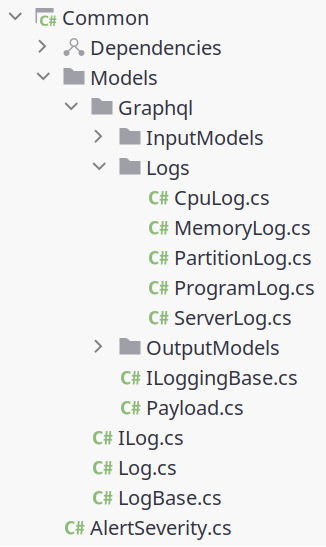
\includegraphics[width=0.4\linewidth]{images/common_structure.png} 
	\caption{Struktura Common projekta}
	\label{slk:common_structure.png}
\end{figure}

\section{ILog.cs}
Glavno sučelje, svaki Log nasljeđuje polja definirana u njemu.

\section{Graphql direktorij}
Graphql direktorij sadržava klase i sučelja koji se koriste za komunikaciju API i Monitor programa.
Neko od važnijih komponenti direktorija:
\begin{itemize}
	\item Payload.cs - sastoji se od Data polja koje sadržava podatke o poslužitelju koji se vraćaju korisniku te Error polja koje je prazno osim u slučaju pogreške prilikom obrade zahtjeva
	\item InputModels direktorij - sadržava klase koje se koriste prilikom dodavanja ili izmijene podataka. Primjer klase:
	\lstinputlisting[firstline=3,language=CSharp,title=CpuInput.cs]{Common/Models/Graphql/InputModels/CpuInput.cs}
	\item Logs direktorij - sadržava klase koje opisuju Log podatke za određen aspekt poslužitelja
	\item OutputModels direktorij - sadržava klase koje se koriste prilikom vraćanja API odgovora. Primjer klase:
	\lstinputlisting[firstline=5,language=CSharp,title=MemoryOutput.cs]{Common/Models/Graphql/OutputModels/MemoryOutput.cs}
\end{itemize}

\chapter{Web stranica}
Web stranica je napravljena pomoću \ref{pog:vue} Vue frameworka.

\section{public/index.html}
Koristi se Vue framework te se zbog toga koristi samo jedna HTML stranica, u kojoj se prikazuju renderirane komponente.

\section{App.vue}
Glavna .vue datoteka koja kontrolira sadržaj koji se prikazuje, stvara se prilikom pokretanja programa.

\section{src/components direktorij}
Vue framework koristi komponente kako bi se dijelovi koda mogli ponovno koristiti. Sve komponente se nalaze u ovom direktoriju. Primjer dijela jedne takve komponente:
\lstinputlisting[language=Javascript,firstline=45,title=MemoryInfo.vue]{website/src/components/MemoryInfo.vue}

\section{src/models direktorij}
Models direktorij sadržava klase koje se koriste za pohranjivanje podataka dohvaćenih s API-a. Primjer klase:
\lstinputlisting[firstline=3,language=Javascript,title=Partition.ts]{website/src/models/Partition.ts}

\section{api.ts}
Zadužen za dohvaćanje podataka s API-a. Primjer dohvaćanja podataka o procesoru za trenutni server:
\lstinputlisting[title=getCpu(),firstline=27,lastline=53,language=Javascript]{website/src/api.ts}

\section{ChartHelper.ts}
Pomoćna datoteka koja se koristi za pretvorbu podataka koje API vraća u točke na grafu.

%--- LITERATURA / REFERENCES ---------------------------------------------------

% Literatura se automatski generira iz zadane .bib datoteke / References are automatically generated from the supplied .bib file
% Upiši ime BibTeX datoteke bez .bib nastavka / Enter the name of the BibTeX file without .bib extension
\bibliography{literatura}



%--- SAŽETAK / ABSTRACT --------------------------------------------------------

% Sažetak na hrvatskom
\begin{sazetak}
  Unesite sažetak na hrvatskom.
\end{sazetak}

\begin{kljucnerijeci}
  prva ključna riječ; druga ključna riječ; treća ključna riječ
\end{kljucnerijeci}


% Abstract in English
\begin{abstract}
  Enter the abstract in English.
  
\end{abstract}

\begin{keywords}
  the first keyword; the second keyword; the third keyword
\end{keywords}


%--- PRIVITCI / APPENDIX -------------------------------------------------------

% Sva poglavlja koja slijede će biti označena slovom i riječi privitak / All following chapters will be denoted with an appendix and a letter
\backmatter

\chapter{The Code}


\end{document}
